\begin{Exercise}[label = trinity, origin = Aaron Wild, title = {Project Trinity}, difficulty = 3]
	\hspace{0.02pt}
	Die Ausbreitung einer halbkreisförmigen Schockwelle hängt von der Energie $E$ der Explosion sowie der Dichte der Luft $\rho$ ab.
	\Question Bestimme eine Gleichung, die den Radius $R$ der Schockwelle als Funktion der Zeit $t$ nach der Explosion angibt.
	\ExeText Die folgenden Bilder zeigen die Schockwelle nach dem ersten Atombombentest der USA 1945, \textit{Project Trinity}:
		\begin{figure}[h]
		\begin{subfigure}[b]{0.5\textwidth}
			\centering
			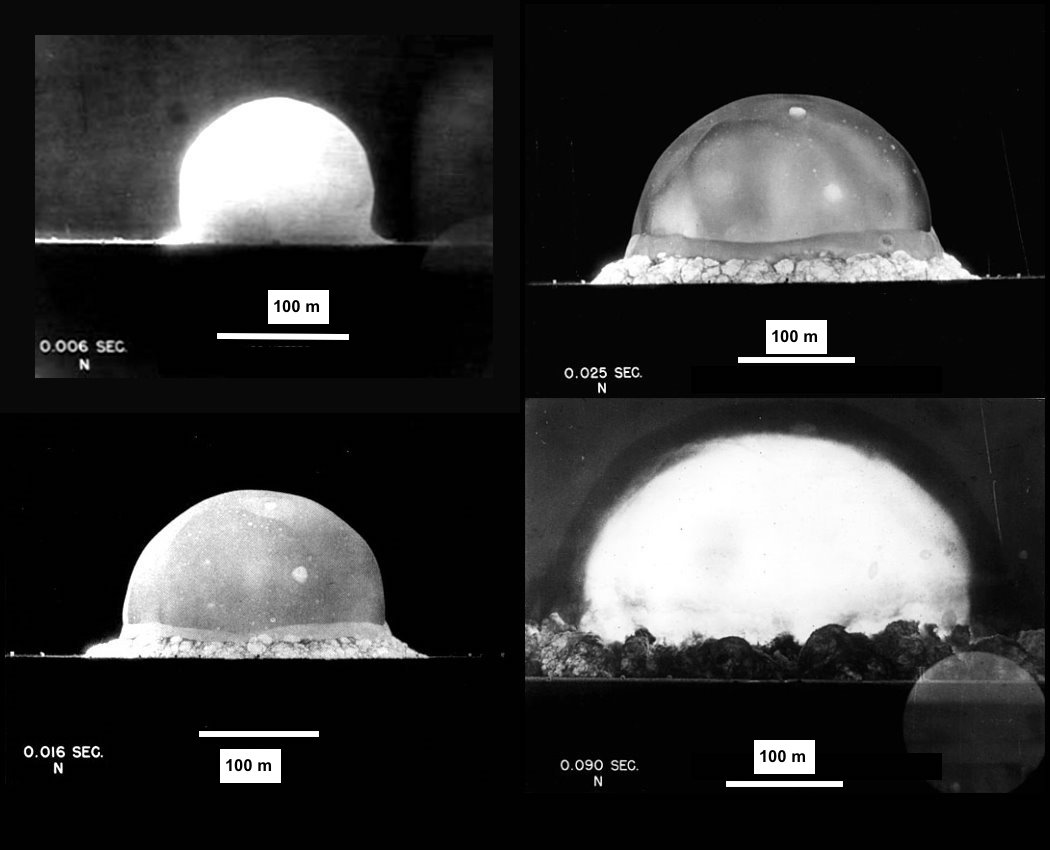
\includegraphics[scale = 0.2]{../tasks/selfmade/trinityim.jpeg}
		\end{subfigure}
		\begin{subfigure}[b]{0.5\textwidth}
			\centering
			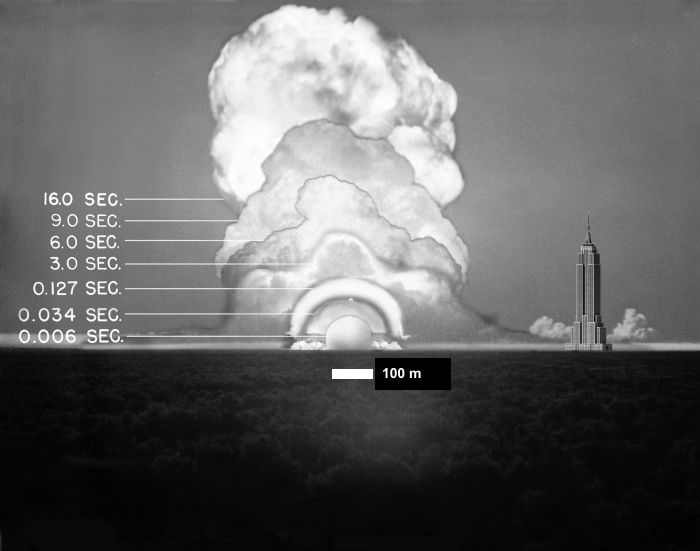
\includegraphics[scale = 0.25]{../tasks/selfmade/trinityim2.png}
		\end{subfigure}
		\caption{Massstabsgerechte Abbildung einer Schockwelle nach der Detonation}
		\label{fig:trinityim}
		\end{figure}
	\Question Unterstützen diese Bilder dein Ergebnis aus 1.?
\end{Exercise}
\begin{Answer}[ref  = trinity]
	\Question Um den Radius als Funktion der Zeit darstellen zu können, reicht es, wenn wir uns fragen, wie man die gegebenen Größen ($E$, $\rho$  und $t$) miteinander multiplizieren muss, damit am Ende eine Größe mit der Einheit eines Radius, also Meter, da steht.\\
	Dazu ist es sinnvoll, sich von den konkreten Einheitensystemen zu lösen, und mit sog. Dimensionen zu rechnen. Diese sind in unserem Fall die Dimensionen der Zeit $T$, der Masse $M$ und der Strecke $M$. Der Vorteil von Dimensionen ist, dass sie uns von willkürlichen Einheiten befreien. Es ist also egal, ob wir eine Masse in Pfund oder Kilogramm angeben, ihre Dimension bleibt immmer die der Masse, $M$. Bei einem Volumen ist es egal, ob wir es in $m^3$ oder in Unzen angeben, die Dimension bleibt immer $L^3$.\\
	Die Dimension der Zeit zu finden ist doch eher einfach, es ist nämlich nur $T$. Für die der Dichte können wir uns die Definitionsgleichung anschauen, $\rho = \nicefrac{m}{V}$. $m$ ist eine Masse, hat also als Dimension $M$; $V$ ist ein Volumen, hat also als Dimension eine Länge im Kubik, $L^3$. Die Energie ist ein wenig schwieriger. Wir wissen aber, dass die Energie definiert ist als Kraft mal Weg ($ E = Fs$), und die Kraft wiederum als Masse mal Beschleunigung ($F = m a$), und die Beschleunigung wiederum ist Geschwindigkeitsänderung pro Zeit ($a = \nicefrac{v}{t}$), und die Geschwindigkeit selber ist Wegänderung pro Zeit ($v=\nicefrac{s}{t}$.) Ab jetzt wird es sinnvoll, sich eine Notation für die Dimension einer Größe auszudenken. Das macht man, indem man die Größe in eckige Klammern packt, also $\left[t\right] = T$ und so weiter. Für die Energie kommen wir, wenn wir all das einfach zusammen packen, auf $\left[E\right] = L^2 \cdot M\cdot T^{-2}$.\\
	Jetzt können wir anfangen, die Aufgabe zu lösen. Dazu können wir zuerst einmal schauen, was passiert, wenn wir $E$, $t$ und $\rho$ einfach ohne nachzudenken brachial zusammen multiplizieren. Nennen wir diese Größe $\nu = Et\rho$. Dann ist deren Dimension gegeben durch
	\begin{equation}\label{trinity:wrongsol}
		\left[\nu \right] = \left[E\right]\cdot \left[t\right]\cdot \left[\rho\right] = L^2\cdot M \cdot T^{-2}\cdot T \cdot M \cdot L^{-3} = L^{-1}\cdot M^2 \cdot T^{-1}.
	\end{equation}
	Wir sehen, dass einfach multiplizieren nicht klappt (Wir erwarten ja $\left[\nu\right] = \left[R\right] = L$)!\\
	Also müssen wir uns einen allgemeineren Ansatz überlegen. Der Ansatz, der am Allgemeinsten ist, ist einfach, irgendwelche Potenzen für die drei Größen anzunehmen ($\alpha$, $\beta$ und $\gamma$), und dann zu schauen, wie man diese wählen muss, damit die Dimensionen aufgehen\footnote[2]{Ab jetzt werden Potenzgesetze wirklich hilfreich!}. In diesem Fall also
	\begin{equation}\label{trinity:dim1}
		\left[R\right] = L \overset{!}{=} \left[E\right]^\alpha\cdot\left[t\right]^\beta\cdot\left[\rho\right]^\gamma = L^{2\alpha} \cdot M^\alpha\cdot T^{-2\alpha}\cdot T^\beta\cdot M^\gamma \cdot L^{-3\gamma} = L^{2\alpha-3\gamma}\cdot M^{\alpha + \gamma} \cdot T^{-2\alpha + \beta}.
	\end{equation}
	Wir wollen jetzt $\alpha$, $\beta$ und $\gamma$ so wählen, dass die Dimension stimmt, also links und rechts des Gleichheitszeichens wirklich auch die gleichen Sachen stehen. Es sollen die drei Exponeten also so gewählt werden, dass $L$ den Exponenten 1 hat, und $M$ und $T$ jeweils null. Daraus können wir ein Gleichungssystem schreiben
	\begin{subequations}\label{trinity:soe}
		\begin{equation}\label{trinity:a1}
			2\alpha - 3\gamma  = 1
		\end{equation}
		\begin{equation}\label{trinity:a2}
			\alpha + \gamma = 0
		\end{equation}
		\begin{equation}\label{trinity:b1}
			-2\alpha + \beta = 0.
		\end{equation}
	\end{subequations}
	Das kann man einfach lösen\footnote[3]{Dazu stellt man am Besten \eqref{trinity:a2} nach $\gamma$ um, $-\alpha = \gamma$, und setzt dann in \eqref{trinity:a1} ein. Da kommt man auf $2\alpha + 3\alpha = 1 \Rightarrow 5\alpha = 1 \Rightarrow \alpha = \nicefrac{1}{5}$. Damit hat man dann sofort $\gamma  = -\alpha = -\nicefrac{1}{5}$ und $\beta = -2\alpha = -\nicefrac{2}{5}$ (über \eqref{trinity:b1})}, und kommt auf $\alpha = \nicefrac{1}{5}$, $\beta = \nicefrac{2}{5}$ und $\gamma = -\nicefrac{1}{5}$, womit $R\left(t\right)$ also gegeben ist durch
	\begin{equation}\label{trinity:rt}
		R\left(t\right) = E^{\nicefrac{1}{5}}\cdot t^{\nicefrac{2}{5}} \cdot \rho^{-\nicefrac{1}{5}} = \sqrt[5]{\frac{Et^2}{\rho}}.
	\end{equation}
	Das Ergebnis ist aber noch nicht vollständig! Was wir durch die Dimensionsanalyse nämlich nicht feststellen können, ist, ob in dem Produkt \eqref{trinity:rt} nicht noch irgendeine Zahl steht (also z.B. $\nicefrac{\pi}{4}$, $30000$ oder $e^{\sqrt{2}}$. ), weil sich dadurch ja die Dimension des Ergebnis nicht ändert. Um die allgemein mögliche Lösung zu finden, müssen wir also schreiben
		\begin{equation}\label{trinity:rtc}
			\boxed{
				R\left(t\right) = c\cdot \sqrt[5]{\frac{Et^2}{\rho}},
				}
		\end{equation}
		wobei $c$ eben diese Konstante ist. Die könenn wir durch die Dimensionsanalyse aber nicht abschätzen (wie auch?). Das stattdessen kann man hier entweder auf experimentelle Daten zurückgreifen, oder aber weitere theoretische Analysen betreiben.
	\Question Da die Bilder massstabsgerecht sind, können wir daraus $R\left(t\right)$ messen, indem wir ein Lineal nehmen (dabei ist es sinnvoll, nach $t=0.127~\mathrm{s}$) aufzuhören. Es ergeben sich folgende Werte
%	\begin{table}[h]
%		\centering
%	\begin{tabular}{|c|c|}
%		\hline
%	$t/\mathrm{s}$	& $R/\mathrm{m}$ \\ 
%		\hline \hline 
%	0.006	& 95.0 \\ 
%		\hline 
%	0.016	& 114.0 \\ 
%		\hline 
%	0.025	& 124.0 \\ 
%		\hline 
%	0.034	& 143.0 \\ 
%		\hline 
%	0.09	&  175.0\\ 
%		\hline 
%	0.127	&  179.0\\ 
%		\hline 
%	\end{tabular} 
%	\caption{Messwerte aus den Abbildungen}
%	\label{trinity:t1}
%\end{table}
	Wir können jetzt schauen, ob diese Messwerte tatsächlich dem Zusammenhang $R\propto \sqrt[5]{t^2}$ entsprechen, wie wir ihn aus \eqref{trinity:rtc} erwarten würden.\\
	Dazu können wir einen Graphen zeichnen. Wenn wir uns aber einfach nur den Graphen $R\left(t\right)$ anschauen, können wir da nicht viel erkennen.
%	\begin{figure}[h]
\centering
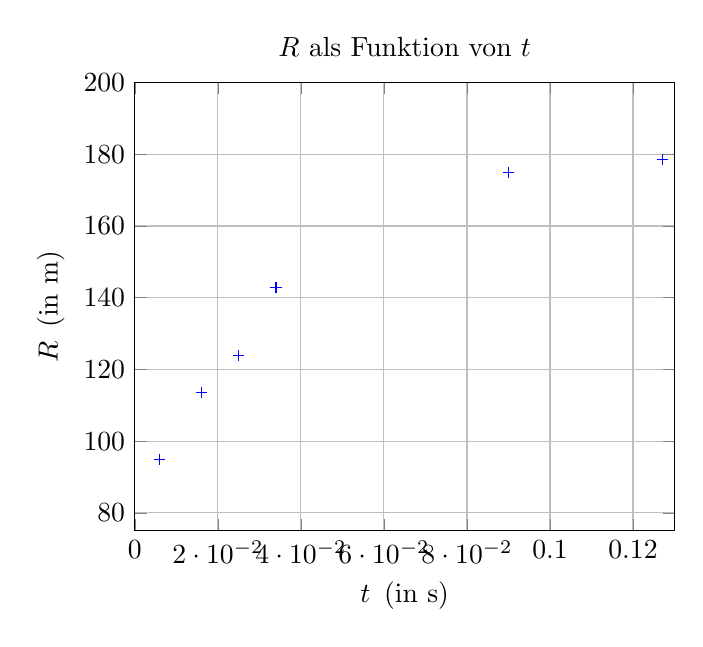
\begin{tikzpicture}
	\begin{axis}[xmin = 0, xmax = 0.13, ymin = 75, ymax = 200, grid = major, xlabel = {$t~\left(\mathrm{in~s}\right)$}, ylabel = $R~\left(\mathrm{in~m}\right)$, title ={ $R$ als Funktion von $t$} ]
%x labels  = {0,0.02,0.04,0.08,0.10,0.12}
\addplot[blue, only marks, mark = +] coordinates
{(0.006, 95.)  (0.025, 123.81) (0.016, 113.636) (0.09, 
	175.) (0.034, 142.857) (0.127, 178.571)
	};

	\end{axis}
\end{tikzpicture}
\end{figure}
	 Viel besser wird es, wenn wir $R^5\left(\sqrt{t}\right)$ zeichnen. Das sollte dann nämlich einfach eine lineare Funktion sein. Danach sieht es auch aus.
	% \begin{figure}[h]
\centering
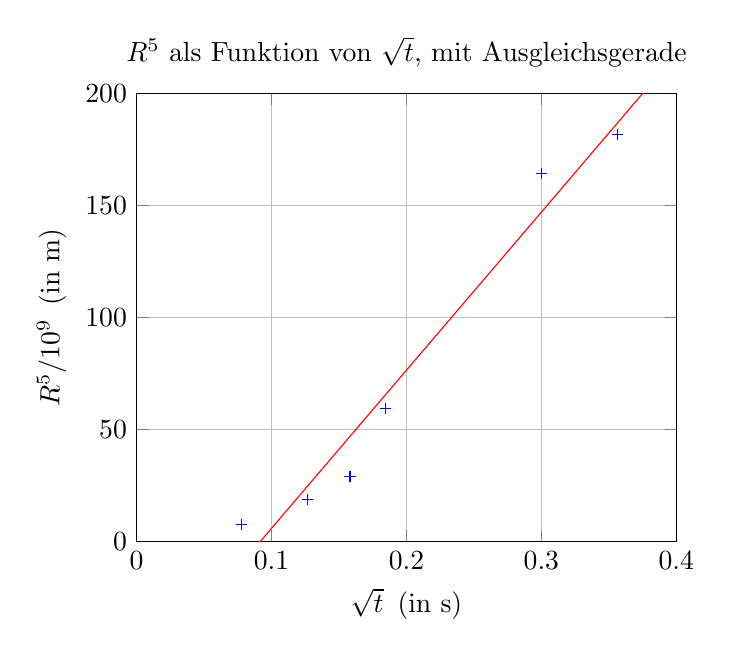
\begin{tikzpicture}
	\begin{axis}[xmin = 0, xmax = 0.4, ymin = 0, ymax = 200, grid = major, xlabel = {$\sqrt{t}~\left(\mathrm{in~s}\right)$}, ylabel = $R^5/10^{9}~\left(\mathrm{in~m}\right)$, title ={ $R^5$ als Funktion von $\sqrt{t}$, mit Ausgleichsgerade} ]

\addplot[blue, only marks, mark = +] coordinates
{(0.0774597, 7.73781) (0.158114, 29.0918) (0.126491, 18.949) (0.3, 
		164.131) (0.184391, 59.499) (0.356371, 181.577)};

\addplot[red] {-64.532+705.153*x};

	\end{axis}
\end{tikzpicture}
\end{figure}
	 Es scheint also, als sei unser Ergebnis aus 1. im Einklang mit diesen Messwerten. Schön ist, dass wir dafür $c$ gar nicht kennen müssen!
\end{Answer}
